\documentclass[
	ngerman,
	ruledheaders=section,   % Ebene bis zu der die Überschriften mit Linien abgetrennt werden, vgl. DEMO-TUDaPub
	class=report,		    % Basisdokumentenklasse. Wählt die Korrespondierende KOMA-Script Klasse
	thesis={type=bachelor}, % Dokumententyp Thesis, für Dissertationen siehe die Demo-Datei DEMO-TUDaPhd
	accentcolor=9c,			% Auswahl der Akzentfarbe
	custommargins=true,    % Ränder werden mithilfe von typearea automatisch berechnet
	marginpar=false,        % Kopfzeile und Fußzeile erstrecken sich nicht über die Randnotizspalte
	% BCOR=5mm,             % Bindekorrektur, falls notwendig
	parskip=half-,          % Absatzkennzeichnung durch Abstand vgl. KOMA-Script
	fontsize=11pt,          % Basisschriftgröße laut Corporate Design ist mit 9pt häufig zu klein
]{tudapub}

% Scala support
\usepackage{listings}
\usepackage{color}

\definecolor{dkgreen}{rgb}{0,0.6,0}
\definecolor{gray}{rgb}{0.5,0.5,0.5}
\definecolor{mauve}{rgb}{0.58,0,0.82}

\lstset{
  language=scala,
  aboveskip=3mm,
  belowskip=3mm,
  showstringspaces=false,
  basicstyle={\small\ttfamily},
  numbers=none,
  numberstyle=\tiny\color{gray},
  keywordstyle=\color{blue},
  commentstyle=\color{dkgreen},
  stringstyle=\color{mauve},
  breaklines=true,
  breakatwhitespace=true,
  tabsize=2,
}
 
% Sprachanpassung & Verbesserte Trennregeln 
\usepackage[english, main=ngerman]{babel}

% Anführungszeichen vereinfacht
\usepackage[autostyle]{csquotes}

% Falls mit pdflatex kompiliert wird, wird microtype automatisch geladen, in diesem Fall muss diese Zeile entfernt werden, und falls weiter Optionen hinzugefügt werden sollen, muss dies über
% \PassOptionsToPackage{Optionen}{microtype} vor \documentclass hinzugefügt werden.
\usepackage{microtype}

% Literaturverzeichnis
\usepackage{biblatex} 
\bibliography{DEMO-TUDaBibliography}
 
% Paketvorschläge Tabellen 
\usepackage{tabularx}    % Tabellen, die sich automatisch der Breite anpassen
\usepackage{booktabs}    % Verbesserte Möglichkeiten für Tabellenlayout über horizontale Linien

% Paketvorschläge Mathematik
% \usepackage{mathtools} % erweiterte Fassung von amsmath
% \usepackage{amssymb}   % erweiterter Zeichensatz
% \usepackage{siunitx}   % Einheiten

% Formatierungen für Beispiele in diesem Dokument. Im Allgemeinen nicht notwendig!
\let\file\texttt
\let\code\texttt
\let\tbs\textbackslash
\let\pck\textsf
\let\cls\textsf

% Zapf-Dingbats Symbole
\usepackage{pifont}
\newcommand*{\FeatureTrue }{\ding{52}}
\newcommand*{\FeatureFalse}{\ding{56}}

\begin{document}

\Metadata{
	title=TUDaThesis - Abschlussarbeiten im CD der TU Darmstadt,
	author=Marei Peischl
}

\title{My Bachelorthesis title}
% \subtitle{No subtitle}
\author[P. Hinz]{Philipp Hinz} % optionales Argument ist die Signatur,
\reviewer{Gutachter 1 \and Gutachter 2 \and noch einer \and falls das immernoch nicht reicht}

% Diese Felder werden untereinander auf der Titelseite platziert.
% \department ist eine notwendige Angabe, siehe auch dem Abschnitt `Abweichung von den Vorgaben für die Titelseite'

% Das Kürzel wird automatisch ersetzt und als Studienfach gewählt, siehe Liste der Kürzel im Dokument.
\department{inf}
\institute{Institut}
\group{Arbeitsgruppe}

\submissiondate{\today}
\examdate{\today}

\maketitle

% oder \affidavit[digital] falls eine rein digitale Abgabe vorgesehen ist.
\affidavit
% Es gibt mit Version 3.20 die Möglichkeit ein Bild als Signatur einzubinden.
% TUDa-CI kann nicht garantieren, dass dies zulässig ist oder eine eigenhändige Unterschrift ersetzt.
% Dies ist durch Studierende vor der Verwendung abzuklären.
% Die Verwendung funktioniert so:
%\affidavit[signature-image={\includegraphics[width=\width,height=1cm]{example-image}}, <hier können andere Optionen wie z.B. affidavit=digital zusätzlich stehen>]

\tableofcontents

\chapter{Introduction}
Modern applications often rely on distributed systems that allow users to collaborate and share data across different devices and networks. One approach to achieve this is to use conflict-free replicated data types (CRDTs), which are data structures that can be replicated and modified concurrently without coordination. CRDTs enable local-first applications, which prioritize local availability and responsiveness over global consistency.

However, CRDTs also pose some challenges for application developers, especially when it comes to authentication and authorization. Authentication is the process of verifying the identity of a user or device, while authorization is the process of granting or denying access rights to resources based on predefined policies. CRDTs do not inherently support authentication or authorization mechanisms, which means that any replica can modify any part of the shared data without restrictions.

However, this also poses some challenges to ensuring the security and privacy of shared data. For example, how can a user verify that another user is who they claim to be? How can a user control who can access their data and what they can do with it? How can a user prevent unauthorized or malicious modifications of their data by other users or devices?

This thesis proposes a novel type of CRDTs called ECmRDTs (extendable conflict-free replicated data types), which allows us to write extensions enabling authentication and authorization in local-first applications. We use symmetric and assymetric encryption techniques to protect the confidentiality and integrity of shared data, as well as to enforce access control policies based on proofs provided by users. 

To demonstrate the feasibility and applicability of ECmRDTs, this thesis presents a case study of a rating application called Ratable as its underlying data model. The case study also requires a new type of architecture that supports local-first principles and enables efficient synchronization of encrypted data among replicas. This thesis introduces several concepts and techniques that can help design and implement such an architecture.

\section{CRDT}
Conflict-free replicated data types (CRDTs) are data structures that can be replicated across multiple nodes in a distributed system, and can be updated concurrently without coordination or locking. CRDTs guarantee eventual consistency, meaning that all replicas will converge to the same state if no new updates are made. CRDTs are useful for applications that require high availability, low latency and tolerance to network partitions.

There are two main approaches to CRDTs: state-based (CvRDT) and operation-based (CmRDT). In state-based CRDTs, each replica maintains a full copy of the data structure, and updates are propagated by sending the entire state or a delta-state to other replicas. The merge function for state-based CRDTs must be commutative, associative and idempotent, ensuring that the order and number of merges do not affect the final state. In operation-based CRDTs, each replica maintains a partial copy of the data structure, and updates are propagated by sending only the operations that modify the state to other replicas. The delivery function for operation-based CRDTs must ensure causal order, meaning that an operation cannot be applied before its dependencies are satisfied. The operations for operation-based CRDTs must also be commutative, ensuring that the order of concurrent operations does not affect the final state.

In this thesis, we will use operation-based CRDTs to build extendable CRDTs (ECmRDTs), which are CRDTs that can dynamically incorporate new data types and operations without requiring a global agreement or a system restart. We will show how ECmRDTs can support various use cases such as collaborative editing, online gaming and social networking.

\chapter{Case Study}
Our case study is named Ratable. With Ratable users can create ratable objects and let a group of people rate them. Ratable is an application, users can interact with on their mobile devices or desktop computers. 

The core idea contrary to usual rating services is that not everyone can rate a Ratable. With a newly created Ratable two links are provided. A rate and a view link. Only people with the rate link can rate and view the ratable.

Ratable is implemented as a cloud-native local-first application. Ratable allows users to use the application without an internet connection and provides updates/changes in real-time. This provides for a very fluent usage of Ratable because we do not need to have any loading screens. The only time we need to load something is when we access some Ratable for the first time. Changes to Ratables are done instantly and synchronized when possible.

Cloud-native and local-first are two design principles that enable Ratable to deliver a fast and reliable user experience. Cloud-native means that Ratable is built and deployed using cloud computing services, such as storage, databases, and serverless functions. This allows Ratable to scale up or down according to the demand, and to benefit from the security and availability of the cloud providers. Local-first means that Ratable stores and processes data on the user’s device, rather than on a remote server. This allows Ratable to work offline, and to sync data with the cloud only when needed. This reduces the network latency and bandwidth consumption, and enhances the privacy and autonomy of the user. By combining cloud-native and local-first, Ratable achieves a balance between performance and functionality, and offers a smooth and seamless user experience.

Especially important for local-first applications is the feature that all trust is given to individual users instead of a server. This means that the server for Ratable plays only a secondary role and does not do much more than distributing state. All authorization and authentication are done by the clients themselves. This allows us to enable end-to-end encryption of the state.

\chapter{Extendable CmRDT}
In this chapter, we will look into what ECmRDT's are, what they are trying to do and how they are used to achieve the goal.

\section{Overview}
CmRDTs are operation-based CRDTs that allow concurrent updates on replicated data without coordination. However, CmRDTs have some limitations, such as the lack of security and the difficulty of adding new features. To overcome these limitations, we introduce ECmRDTs, which are extendable CmRDTs that support extensions for verification, mutation, interaction, and authentication of events and state.

An event is an operation that modifies the state of an ECmRDT. A state is the current value of an ECmRDT. Events are signed by the clients that generate them and sent to a server that stores them. The server acts as an event source, which means that it provides events to clients on demand. Clients can request events from the server and apply them to their local state to update their ECmRDTs. This way, clients do not need to store events locally and can always access the latest version of the data.

Extensions are functions that can be attached to an ECmRDT to enhance its functionality. Extensions can be defined in a pipeline, which is a sequence of extensions that are applied to an event before it is applied to the state. Extensions can perform various tasks, such as:

\begin{itemize}
  \item Verifying the replicaId of an event to ensure its origin
  \item Changing some variables in the state before or after applying an event
  \item Migrating events from one format to another
  \item Authenticating and authorizing events based on some criteria
\end{itemize}

The main advantage of ECmRDTs is that they enable developers to create secure and customizable data types that can be easily extended with additional functionality. For example, one can use extensions to implement access control policies or data validation rules for an ECmRDT. Extensions can also interact with other extensions and exchange information or modify each other’s behavior.

In summary, ECmRDTs are a novel approach to extend CmRDTs with security and customization features using extensions. Extensions are functions that can verify and mutate events and state in a pipeline. They can also interact with other extensions and authenticate and authorize events based on some criteria. Events are signed operations that modify the state of an ECmRDT and are stored on a server that acts as an event source. Clients can request events from the server and apply them to their local state to update their ECmRDTs.

Lets say we want to implement a counter that can only be incremented by the owner. We would first define the state as a integer counter and one event that increments the state counter by one. The context and generally how these concepts relate to each other will be covered in the next section.

\begin{lstlisting}
    
case class Counter(
  val value: Int,
) 

case class CounterContext(
  val replicaId: ReplicaId,
)  extends IdentityContext

sealed trait CounterEvent extends Event[Counter, CounterContext]

case class AddCounterEvent() extends CounterEvent:
  def asEffect =
    (state, context, meta) => EitherT.pure(
      state.copy(value = state.value + 1)
    )

\end{lstlisting}

Then we would enable an build-in extensions that only lets events pass when they are send by the owner of the ratable.

\begin{lstlisting}

object Counter:
  given EffectPipeline[Counter, CounterContext] = EffectPipeline(
    SingleOwnerEffectPipeline()
  )

\end{lstlisting}

Using only a few lines of code we have now a secure incrementable counter that can only be incremented by the owner. This counter can now be used like the following. The example will first create a replicaId and an initial state. With both we can create a event and apply it to our created state. In the end we print the state before and after applying our event.

\begin{lstlisting}
    
def main(using Crypt) = 
  for
    // Step 1: Create replicaId
    replicaId <- EitherT.liftF(PrivateReplicaId())

    // Step 2: Create initial state.
    counter = ECmRDT[Counter, CounterContext, CounterEvent](Counter(0))

    // Step 3: Create event.
    eventPrepared = counter.prepare(
      AddCounterEvent(),
      CounterContext(replicaId)
    )

    // Step 4: Verify and advance state.
    newCounter <- counter.effect(eventPrepared, MetaContext(
      AggregateId.singleton(replicaId), 
      replicaId
    ))

  yield
    println(s"Old counter: ${counter.state.value}")    // 0
    println(s"New counter: ${newCounter.state.value}") // 1

\end{lstlisting}

How exactly the ECmRDT's and the SingleOwnerEffectPipeline work will be in the next section.

\section{Concepts}

This section explains the main ideas of our ECmRDT with definitions, code examples and how they are connected.

\minisec{Aggregate}

An aggregate is a group of related objects that we handle as one unit when we change data. Each aggregate has a root and a boundary. The boundary shows what is inside the aggregate. The root is one specific object in the aggregate. 

In general, an aggregate is a domain concept where only one aggregate at a time should be changed by a use case. We will define one ECmRDT for each aggregate.

\minisec{ReplicaId}
The ReplicaId is a unique identifier for a user. The ReplicaId has a public/private key pair. With this, we can sign and verify events sent by a user. Because the private key only exists in the corresponding replica as a privateReplicaId, the ReplicaId only has the public key for identification. More details about the ReplicaId are in the chapter about authentication and authorization.

\begin{lstlisting}
case class ReplicaId(
  val publicKey: BinaryData
)
\end{lstlisting}

\minisec{AggregateId}
The AggregateId is a unique identifier for an ECmRDT/aggregate. The AggregateId is a combination of a ReplicaId and random bytes. The ReplicaId in the aggregateId shows the owner of the aggregate. We need to store the ReplicaId to stop other replicas from creating aggregates with the same AggregateId on purpose. The random bytes are used to avoid collisions of AggregateIds within a group of aggregates of a replica.

\begin{lstlisting}
case class AggregateId(
  val replicaId: ReplicaId,
  val randomBytes: BinaryData
)
\end{lstlisting}

\minisec{Effect}
An Event can be converted to an Effect to apply the Event to the state. Generally Effect is a function that takes a state, an context, an MetaContext and returns a new state or an RatableError in future. By returning an RatableError we can abort the Event and therefore verify the Event together with the given parameters if they are valid. The effect is an asynchronous operation because we sometimes need to use cryptographic operations to check the event which are done in web browsers asynchronously.

\begin{lstlisting}
type Effect[A, C] = (A, C, MetaContext) => EitherT[Future, RatableError, A]
\end{lstlisting}

\minisec{Event}
Events are made by users to change the state. Usually events are caused directly by user actions. Events are linked with a context. So events have information specific to one particular event and the context has information that is contained in every event. Events can be changed into effects to be used later to update the state.

\begin{lstlisting}
trait Event[A, C]:
  def asEffect: Effect[A, C]
\end{lstlisting}

\minisec{MetaContext}
MetaContexts contain information required for ECmRDTs but that are not stored directly in the ECmRDT. Currently it contains information about the AggregateId of the ECmRDT and the ReplicaId of the aggregate owner. The reason why dont store the aggregate owner inside the ECmRDT is because we can already get it implicitly from the aggregateId.

The need for MetaContexts comes from the problem on how to initialize ECmRDTs through an initial events and especially how to verify initial events. At creation time when processing the first event the state is yet empty/default initialized. Therefore we would normally not be able to validate the event through the provided state. Using the MetaContext or to be more precise the owner replicaId inside the MetaContext we can enforce the rule to only allow initial events to be sent by the owner of the aggregate.

\begin{lstlisting}
case class MetaContext(
  val aggregateId: AggregateId,
  val ownerReplicaId: ReplicaId,
)
\end{lstlisting}

\minisec{ECmRDTEventWrapper}
Events are implicitly associated with Contexts. This association becomes explicit through an ECmRDTEventWrapper. The reason why we normally only associate Events implicitly is because an ECmRDTEventWrapper contains additional information that is aquired by preparing an Event and Context through an ECmRDT. Only after preparation and conversion to an ECmRDTEventWrapper can it be used to update an ECmRDT. 

The currently primary information packed additionally with an ECmRDTEventWrapper is time. An ECmRDT uses a VectorClock to prevent Event duplicates. The time from the VectorClock is then stored inside the Event to associate it with the time.

\begin{lstlisting}
case class ECmRDTEventWrapper[A, C, +E <: Event[A, C]](
  val time: Long,
  val event: E,
  val context: C,
)
\end{lstlisting}

\minisec{Context}
Events only contain information specific to the aggregate and the information are neither accessible by ECmRDT nor Extensions. Therefore we use Contexts to provide common information stored with events that allow us to use them in ECmRDTs and Extensions. 

A good example is the IdentityContext containing an replicaId. It is used in ECmRDTs to update the VectorClock of the replica sending the Event and also used when filtering Events for Authentication and Authorization.

It should be noted that validation of the IdentityContext itself (if the replicaId is actually the sender) is done outside of the ECmRDT. The validation happens through an signature added to events which can then be verified by the public key inside the replicaId.

\begin{lstlisting}
trait IdentityContext:
	def replicaId: ReplicaId
\end{lstlisting}

\minisec{ECmRDT}
The core concept is the ECmRDT. The ECmRDT consists of a state and a clock. The state contains the actual data of the aggregate. The clock is a VectorClock to prevent duplications of Events. Our ECmRDT does neither handle distribution of Events nor storing pending Events nor validation of identities (see Context section). This has to be done by the user of the ECmRDT.

Our ECmRDT supports two operations. One to prepare an Event and one to apply an prepared event. The prepare operation is used to aquire additional information from the ECmRDT, specifically the clock and bundle the event with an context into one ECmRDTEventWrapper. The apply operation is used to apply the Event to the ECmRDT while also advancing the vector clock.

\begin{lstlisting}
case class ECmRDT[A, C <: IdentityContext, E <: Event[A, C]](
	val state: A,
	val clock: VectorClock = VectorClock(Map.empty)
):
	def prepare(
		event: E, context: C
	)(
		using effectPipeline: EffectPipeline[A, C]
	): ECmRDTEventWrapper[A, C, E] = ...

	def effect(
		wrapper: ECmRDTEventWrapper[A, C, E], meta: MetaContext
	)(
		using effectPipeline: EffectPipeline[A, C]
	): EitherT[Future, RatableError, ECmRDT[A, C, E]] = ...
\end{lstlisting}

\minisec{EffectPipeline}
Extensions are implemented by transforming an Effect to a new Effect. The function that transforms this Effect is called EffectPipeline. EffectPipelines are specified by aggregates to enable extensions to add functionality like logging, validation, mutation or more. Important is that the functionality provided by EffectPipelines is will be used for all Events of an ECmRDT. 

\begin{lstlisting}
trait EffectPipeline[A, C]:
	def apply(effect: Effect[A, C]): Effect[A, C]
\end{lstlisting}

\section{Extensions}
Extensions allow developers to define functionality used in the whole aggregate. Extensions can enable things like event validation, state mutation, replace/adjust State, Context or MetaContext parameters and more. Additionally, Extensions also allow for easier code reuse between aggregates and Extensions can build on existing Extensions. An Extension consists of a EffectPipeline and optionally of a Context and State. 

An EffectPipeline itself is only a function transforming an Effect which itself is a function. The idea now is to intercept the Effect function call and execute custom logic before or after the call. If an aggregate wants to define multiple Extensions we can chain these EffectPipelines into a call chain which results in a single resulting functions which itself is again a EffectPipeline. This does in practice look like the following. Here we log the replicaId of the sender.

\begin{lstlisting}

object TestEffectPipeline:
  def apply[A, C <: IdentityContext](): EffectPipeline[A, C] =
    effect => (state, context, meta) => 
      for
        newState <- effect(state, context, meta)
      yield
        println(s"Sender replicaId: \${context.replicaId}")
        newState

\end{lstlisting}

For the most important feature is that an Effect can also fail. Because of that we are able to shortcircuit the Extension call chain when an error happens or some validation fails. One example for this is the SingleOwnerEffectPipeline. Here we validate that the Context replicaId (event sender replicaId) is the same as the meta replicaId (aggregate owner replicaId). If the check fails we do not continue in calling the given Effect. To make development easier because verification Extensions are common we are using a verifyEffectPipeline helper function. This helper function only expects a list of errors as return. If the list is empty we succeeded and continue the Effect call.

\begin{lstlisting}
  
object SingleOwnerEffectPipeline:
  def apply[A, C <: IdentityContext](): EffectPipeline[A, C] =
    verifyEffectPipeline[A, C]((state, context, meta) => List(
      Option.when(meta.ownerReplicaId != context.replicaId)(
        RatableError(s"Replica ${context.replicaId} is not the owner ${meta.ownerReplicaId} of this state.")
      )
    ))

// Helper to build a synchronous verify only effect pipelines
def verifyEffectPipeline[A, C](
  f: (A, C, MetaContext) => List[Option[RatableError]]
): Effect[A, C] => Effect[A, C] =
  verifyEffectPipelineFuture((a, c, m) => f(a, c, m).map(OptionT.fromOption(_)))
  
// Helper to build a asynchronous verify only effect pipelines
def verifyEffectPipelineFuture[A, C](
  f: (A, C, MetaContext) => List[OptionT[Future, RatableError]]
): Effect[A, C] => Effect[A, C] =
  (effect) =>
    (state, context, meta) => 
      for
        _ <- f(state, context, meta).map(_.toLeft(())).sequence
        newState <- effect(state, context, meta)

      yield
        newState

\end{lstlisting}

In the previous example we have used the IdentityContext by specifying type bounds. Additionally to defining EffectPipelines, Extensions can also define their own Context as well as their own state. When an aggregate wants to use an Extension it has to include the Extension Context and State into its own Context and State. Because of the type bounds we would get a type error if forgotten. How custom Context and State can be used to create more flexible functions will be shown in the section about Authentication and Authorization.

\section{Authentication and authorization}
In this section we will look into what assumptions are met and how a Extension for ECmRDTs is created to enable authentication and authorization. Our goal is that aggregates can define a list of permissions. Certain events may require permissions conditionally as specified by the aggregate. User then need to add proofs for the permissions so that every other user can verify it. 

Proofs are implemented as signatures of a replicaId (the user who wants to use the event) using asymmetric encryption. This also means, that a proof only allows a single user to use an event. For other users new proofs have to be created. The public key of a proof is called a claim and the private key is called a prover. Claims are stored publicly in the aggregate state so that every user is able to verify incoming events.

\begin{lstlisting}
case class Claim[I](
  val publicKey: BinaryData,
  val id: I, // I is a enum value representing the permission
)

case class ClaimProof[C](
  val proof: BinaryData,
  val id: C,
):
  def verify(claim: Claim[C], replicaId: ReplicaId) // ...

case class ClaimProver[ID](
  val privateKey: BinaryData,
  val id: ID
):
  def prove(replicaId: ReplicaId) // ...

\end{lstlisting}

Claims and provers are created using the initial event but the provers are usually not stored inside the aggregate. The only exception is an additional extension called ClaimBehindPassword which tries to reduce the key size that has to be transmitted. The idea is to store the private keys encrypted symmetrically publicly in the aggregate with a shorter password. Now everyone who has the password can create their own proofs.

For this whole system to work we need to make sure that every event telling it was send by an replicaId is actually send by this replicaId. This is important because when validating proofs we verify a signature containg the sender replicaId. If one would be able to spoof the sender replicaId we could use an existing proof send by a different user (that is possible because proofs are public by default because everyone needs to be able to verify them) and spoof their replicaId. Users would then not be able to verify the event correctly. 

This issue is the main reason why the replicaId is a public key where only the user itself does know the private key. Events are signed using the private key so that everyone receiving events from a replicaId can be sure that the replicaId used in the event are legitimit.

\minisec{Extension}
The Extension is implemented using a Context, a State and a EffectPipeline. In the Context we store all the proofs containg the signatures added by the user using an event and in the state we store all claims containing the public key to verify the claims. ClaimProvers are not directly part of the extension and have to be handled by the developers using the Extension.

\begin{lstlisting}
trait AsymPermissionContextExtension[I]:
  def proofs: List[ClaimProof[I]]

  def verifyPermission[A](permission: I): EitherT[Future, RatableError, Unit] = EitherT.cond[Future](
    proofs.exists(_.id == permission), (),
    RatableError(s"Missing permission \$permission.")
  )

trait AsymPermissionStateExtension[I]:
  def claims: List[Claim[I]]
\end{lstlisting}

The State and Context now are used inside the EffectPipeline. The idea is to verify all proofs contained in the Event Context, no matter if they are actually required by the Event. The Extension itself does not even need to know what proofs are required, it only makes sure that all provided proofs are in fact valid. The Effect of the Event itself later can call the verifyPermission method of the Context to easily make sure that alle required permissions are proofed by the context.

So in the EffectPipeline we first have to find the Claim for the respective Proof and then make sure it is valid. If either the claim does not exist or the proof is invalid we cancel the pipeline call chain by returning an error. For this we are using the verifyEffectPipelineFuture helper.

\begin{lstlisting}
object AsymPermissionEffectPipeline:
  def apply[
    A <: AsymPermissionStateExtension[I], 
    I, 
    C <: AsymPermissionContextExtension[I] with IdentityContext
  ](using Crypt): EffectPipeline[A, C] =
    verifyEffectPipelineFuture[A, C]((state, context, meta) =>
      for
        proof <- context.proofs
      yield
        state.claims.find(_.id == proof.id) match
          case Some(claim) => 
            OptionT(proof
              .verify(claim, context.replicaId)
              .map(Option.unless(_)(RatableError("Proof is invalid.")))
            )

          case None => 
            OptionT.pure(RatableError("Claim does not exist."))
    )
\end{lstlisting}

How this extension can be used will be shown in the next section where we will look into how ECmRDTs are used to model the Ratable domain.

\section{Integration into Ratable}
Ratable itself has a simple domain. A Ratable is an object containing a title, categories and ratings. To enable authorization we are using the AsymPermissionExtension with the provided EffectPipeline and to allow easier sharing of private keys we use the ClaimByPasswordExtension. The context provides no custom information and contains the standard IdentityContext as well as the AsymPermissionExtension context.

\begin{lstlisting}
case class Ratable(
  val claims: List[Claim[RatableClaims]],
  val claimsBehindPassword: Map[RatableClaims, BinaryDataWithIV],

  val title: String,
  val categories: Map[Int, Category],
  val ratings: Map[ReplicaId, Rating]
)

case class Rating(
  val ratingForCategory: Map[Int, Int]
)

case class Category(
  val title: String
)

object Ratable:
  given (using Crypt): EffectPipeline[Ratable, RatableContext] = 
    EffectPipeline(
      AsymPermissionEffectPipeline[
        Ratable, RatableClaims, RatableContext]
    )

case class RatableContext(
  val replicaId: ReplicaId,
  val proofs: List[ClaimProof[RatableClaims]]
) 
extends IdentityContext 
    with AsymPermissionContextExtension[RatableClaims]
\end{lstlisting}

Additionally, we define our domain around our state to enable better readability and code reuse.

\begin{lstlisting}
case class Ratable(...):
  def rate(
    replicaId: ReplicaId, 
    ratingForCategory: Map[Int, Int]
  ): Ratable = ...

  def categoriesWithRating: Map[Int, (Category, Int)] = ...
\end{lstlisting}

We only need to provide an event called RateEvent and one Claim called CanRate to create or replace a rating.

\begin{lstlisting}
// we need to extend Enum[T] to allow serialization of enum
enum RatableClaims extends Enum[RatableClaims]:
  case CanRate

// sealed base trait to allow serialization
sealed trait RatableEvent extends Event[Ratable, RatableContext]

case class RateEvent(
  val ratingForCategory: Map[Int, Int]
) extends RatableEvent:
  def asEffect: Effect[Ratable, RatableContext] =
    (state, context, meta) =>
      for
        _ <- context.verifyClaim(RatableClaims.CanRate)
        _ <- EitherT.cond(ratingForCategory.size == state.categories.size, (),
          RatableError(s"Rating must contain ${state.categories.size} categories, but ${ratingForCategory.size} given"))
      yield
        state.rate(context.replicaId, ratingForCategory)
\end{lstlisting}

How ECmRDTs can be integrated 

How the ratable domain is designed using ECmRDT

Specific benifits of ECmRDT in Ratable

\chapter{Architecture}

\minisec{Overview}

Ratable provides its services to users as a web application. The web application itself is static and delivered through an CDN. State is managed and distributed through a serverless backend. The communication between the backend and the web application uses either HTTP for synchronous messaging or websockets for asynchronous messaging both with protobuf for encoding. The asynchronous messaging is handled by a pubsub service where the backend service can subscribe to to receive messages. For data storage we use a serverless nosql solution provided by the cloud provider.

\begin{figure}[h]
  \centering
  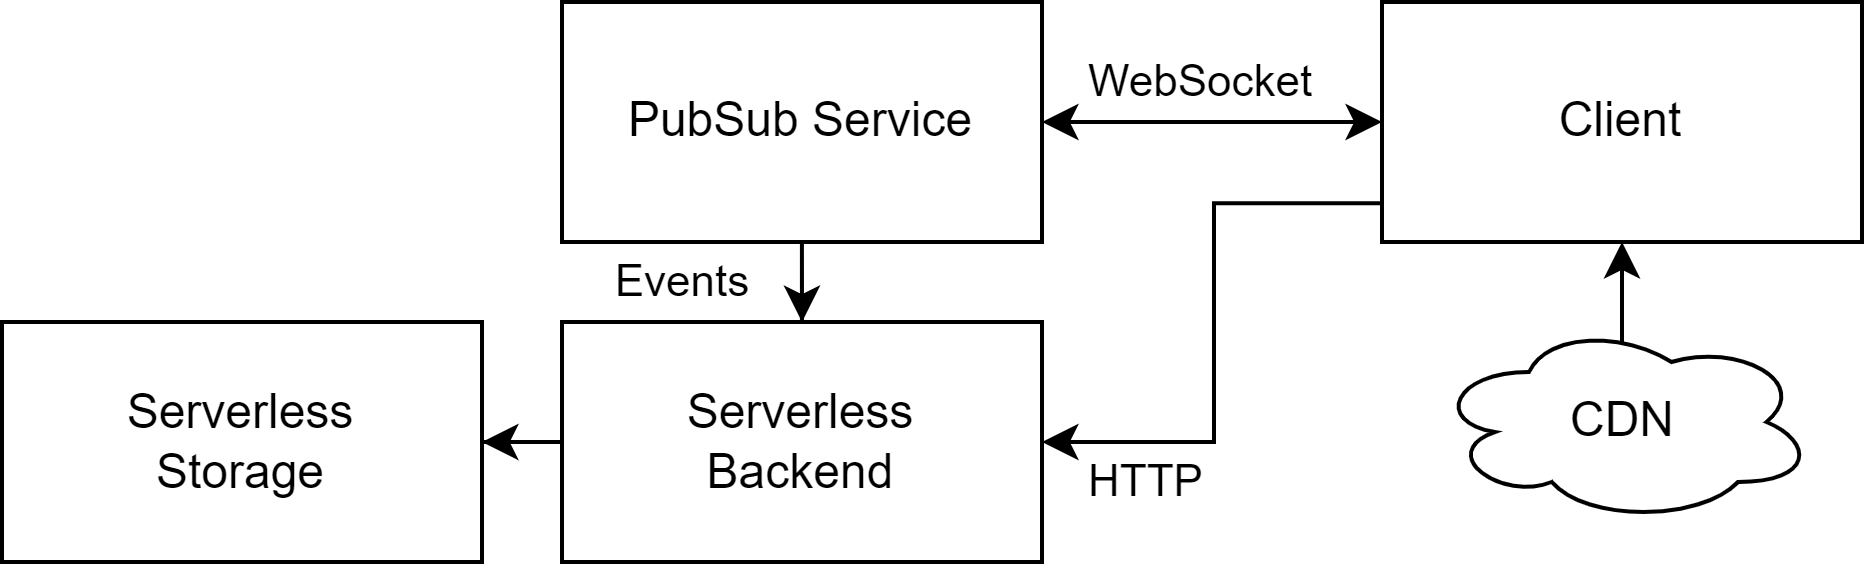
\includegraphics[width=0.7\textwidth]{architecture_services.png}
  \caption{Architecture overview}
\end{figure}

\minisec{Reasoning}

We are providing our services through a web application because the tooling for scala was very good and we could this way provide our services to a larger audience (e.g. mobile and desktop devices) in a more accessable way without downloads. Additionally we provide PWA functionality to enable users to install Ratable as a App on their device. We decided against server side rendering because neither was the tooling for scala was good nor had it a lot of advantages for our use case. Because of this we were able to take a simple and very cost effective (in fact free with our cloud provider) approach in delivering the application to users by giving access to the content files through an CDN. 

We decided to use a serverless backend because it is very cost effective (again free with our cloud provider), is simple to deploy without any system configuration issues while only having the drawback that applications have to be specially designed for a serverless environment. That was not really an issue because we did want to create a cloud-native solution and additionally implemented enough abstraction to be able to change the cloud provider without a complete rewrite. For a similar reason, especially because of the cost-effectiveness we decided to use a serverless nosql storage system. Additionally we decided to use nosql because we did not have specific requirements and the recommmended way by our cloud provider was to use this service. One drawback of serverless that could be brought to consideration are cold start times. Our use-case is not very time-critical and therefore cold starts did not seem to outweight the advantages.

To provide real-time updates we need to have a constant connection to backend. For web applications one would use websockets to implement this feature. Because we are using a general serverless architecture we are not able to simply have a ongoing websocket-conntection to our backend. This issue is solved by a service provided by our cloud provider, the pubsub. Using this service the client can create a websocket connection to the pubsub which is then managed by our backend using events. The backend is called every time a user connects, disconnects or sends a message.

One special thing about our communication is that we are not using json like most web application do but rather are using protobuf. Our messages contain a lot of 'one of' relationships. That means that a lot of messages consist of a type and content in the message where the content contains a sub message. Generally scala has multiple json libraries which support this type of "inheritence" but because of our special case where we do not want to parse the whole type directly (or only with more context) using the given json libraries seemed more difficult than using protobuf where protobuf has extensive support for 'one of' relationships while also providing great scala support. Additionally to note is that we decided with json against storing sub messages simply as string because to store json in json the content first has to be escaped which after mutliple times results in a significant increase of size.

The idea behind ECmRDT would allow us to use peer-to-peer communication instead or additionally to client-server communication. The reason why we decided against it is that it would be out of the scope of this thesis. Implementing peer-to-peer communication would add multiple new problems in implementing the communication, state management and event ordering. It should be noted that theoretically we have indirect peer-to-peer because our server does not do anything more than forwarding all Events.

\section{Project Structure}
Ratable consists of two applications. The serverless backend running accepting messages over HTTP or events over WebSockets and the web application giving an interface to the user and communicating with the backend. Additionally we have a common core module which contains the domain model, the ECmRDT implementation as well as all protobuf definitions modelling the communication between the backend and web application.

Both the web application as well as the backend are structured similarly. They consist of a application and a device layer. Between these two layers can be additional suppo
rtive layers abstracting away the device layer or adding new functionality like a state layer. By using a device layer implementing all interaction with device resources we are able to test the whole application by only mocking this layer. This comes at the cost of having to abstract away every interaction with device resource which can be difficult for more complex apis like database management. 

Layers interact between each other using services. By heavly using dependency injection each service can request the services it needs. Generally services should only request services from the same layer or from a layer below. This is also to prevent cyclic dependencies. 

The application layer is structured differently between the webapp and the backend. In the webapp we decided to use a use case oriented approach. This is useful because it plays nicely with user interactions and the event driven design of ECmRDTs. Here state is managed by its own layer which can then be used in combination with the use cases to drive our user interface. Our user interface is similiar to other frontend frameworks split into pages and components. In the backend the primary goal of the application layer is to provide an entrypoint for all azure functions and then handle all incoming messages. The application layer is split into multiple modules each containing a gateway and multiple message handlers.

\section{State managment}
A core part of this thesis are ECmRDTs. They provide a new way to work with data and therefore state managment is an important part in providing a convient way to work with ECmRDTs. 

We designed the state management in a way that every aggregate defined by a ECmRDT exists as a repository. Aggregates existing only once use the userid as aggregateid enabling theoretical multiuser functionality. The user can either create a new aggregate or load an existing one, it is currently not possible to delete an aggregate. 

An single aggregate is represented by an AggregateView allows a user to listen for changes and submit events. This is the only way to interact with aggregates outside of the state layer.

\begin{lstlisting}
trait AggregateView[A, C, E <: Event[A, C]]:
  def effect(event: E, context: C)(using EffectPipeline[A, C]): EitherT[Future, RatableError, Unit]
  def listen: Signal[A]
\end{lstlisting}

Internally the aggregate is contained by an AggregateFacade. It contains the concrete ECmRDT value and allows free mutations around it. This free ability of free mutations is needed for operations like acknowledging sent events. This additional abstraction is needed because we do not store the ECmRDT directly. We need additional wrappers to enable communication and asynchronous mutations. 

\begin{lstlisting}
class AggregateFacade[A, C <: IdentityContext, E <: Event[A, C]](
  private val initial: EventBufferContainer[A, C, E]
):
  def listen: Signal[EventBufferContainer[A, C, E]] = variable

  def mutate(
    f: EventBufferContainer[A, C, E] => EitherT[Future, RatableError, EventBufferContainer[A, C, E]]
  ): EitherT[Future, RatableError, EventBufferContainer[A, C, E]] = ???

\end{lstlisting}

These AggregateFacades are then created and cached by the AggregateFacadeProvider so that only one exists per aggregate at any moment. Around the AggregateFacadeProvider we have the AggreagteViewProvider which converts AggregateFacades into AggregateViews. 

\begin{figure}[h]
  \centering
  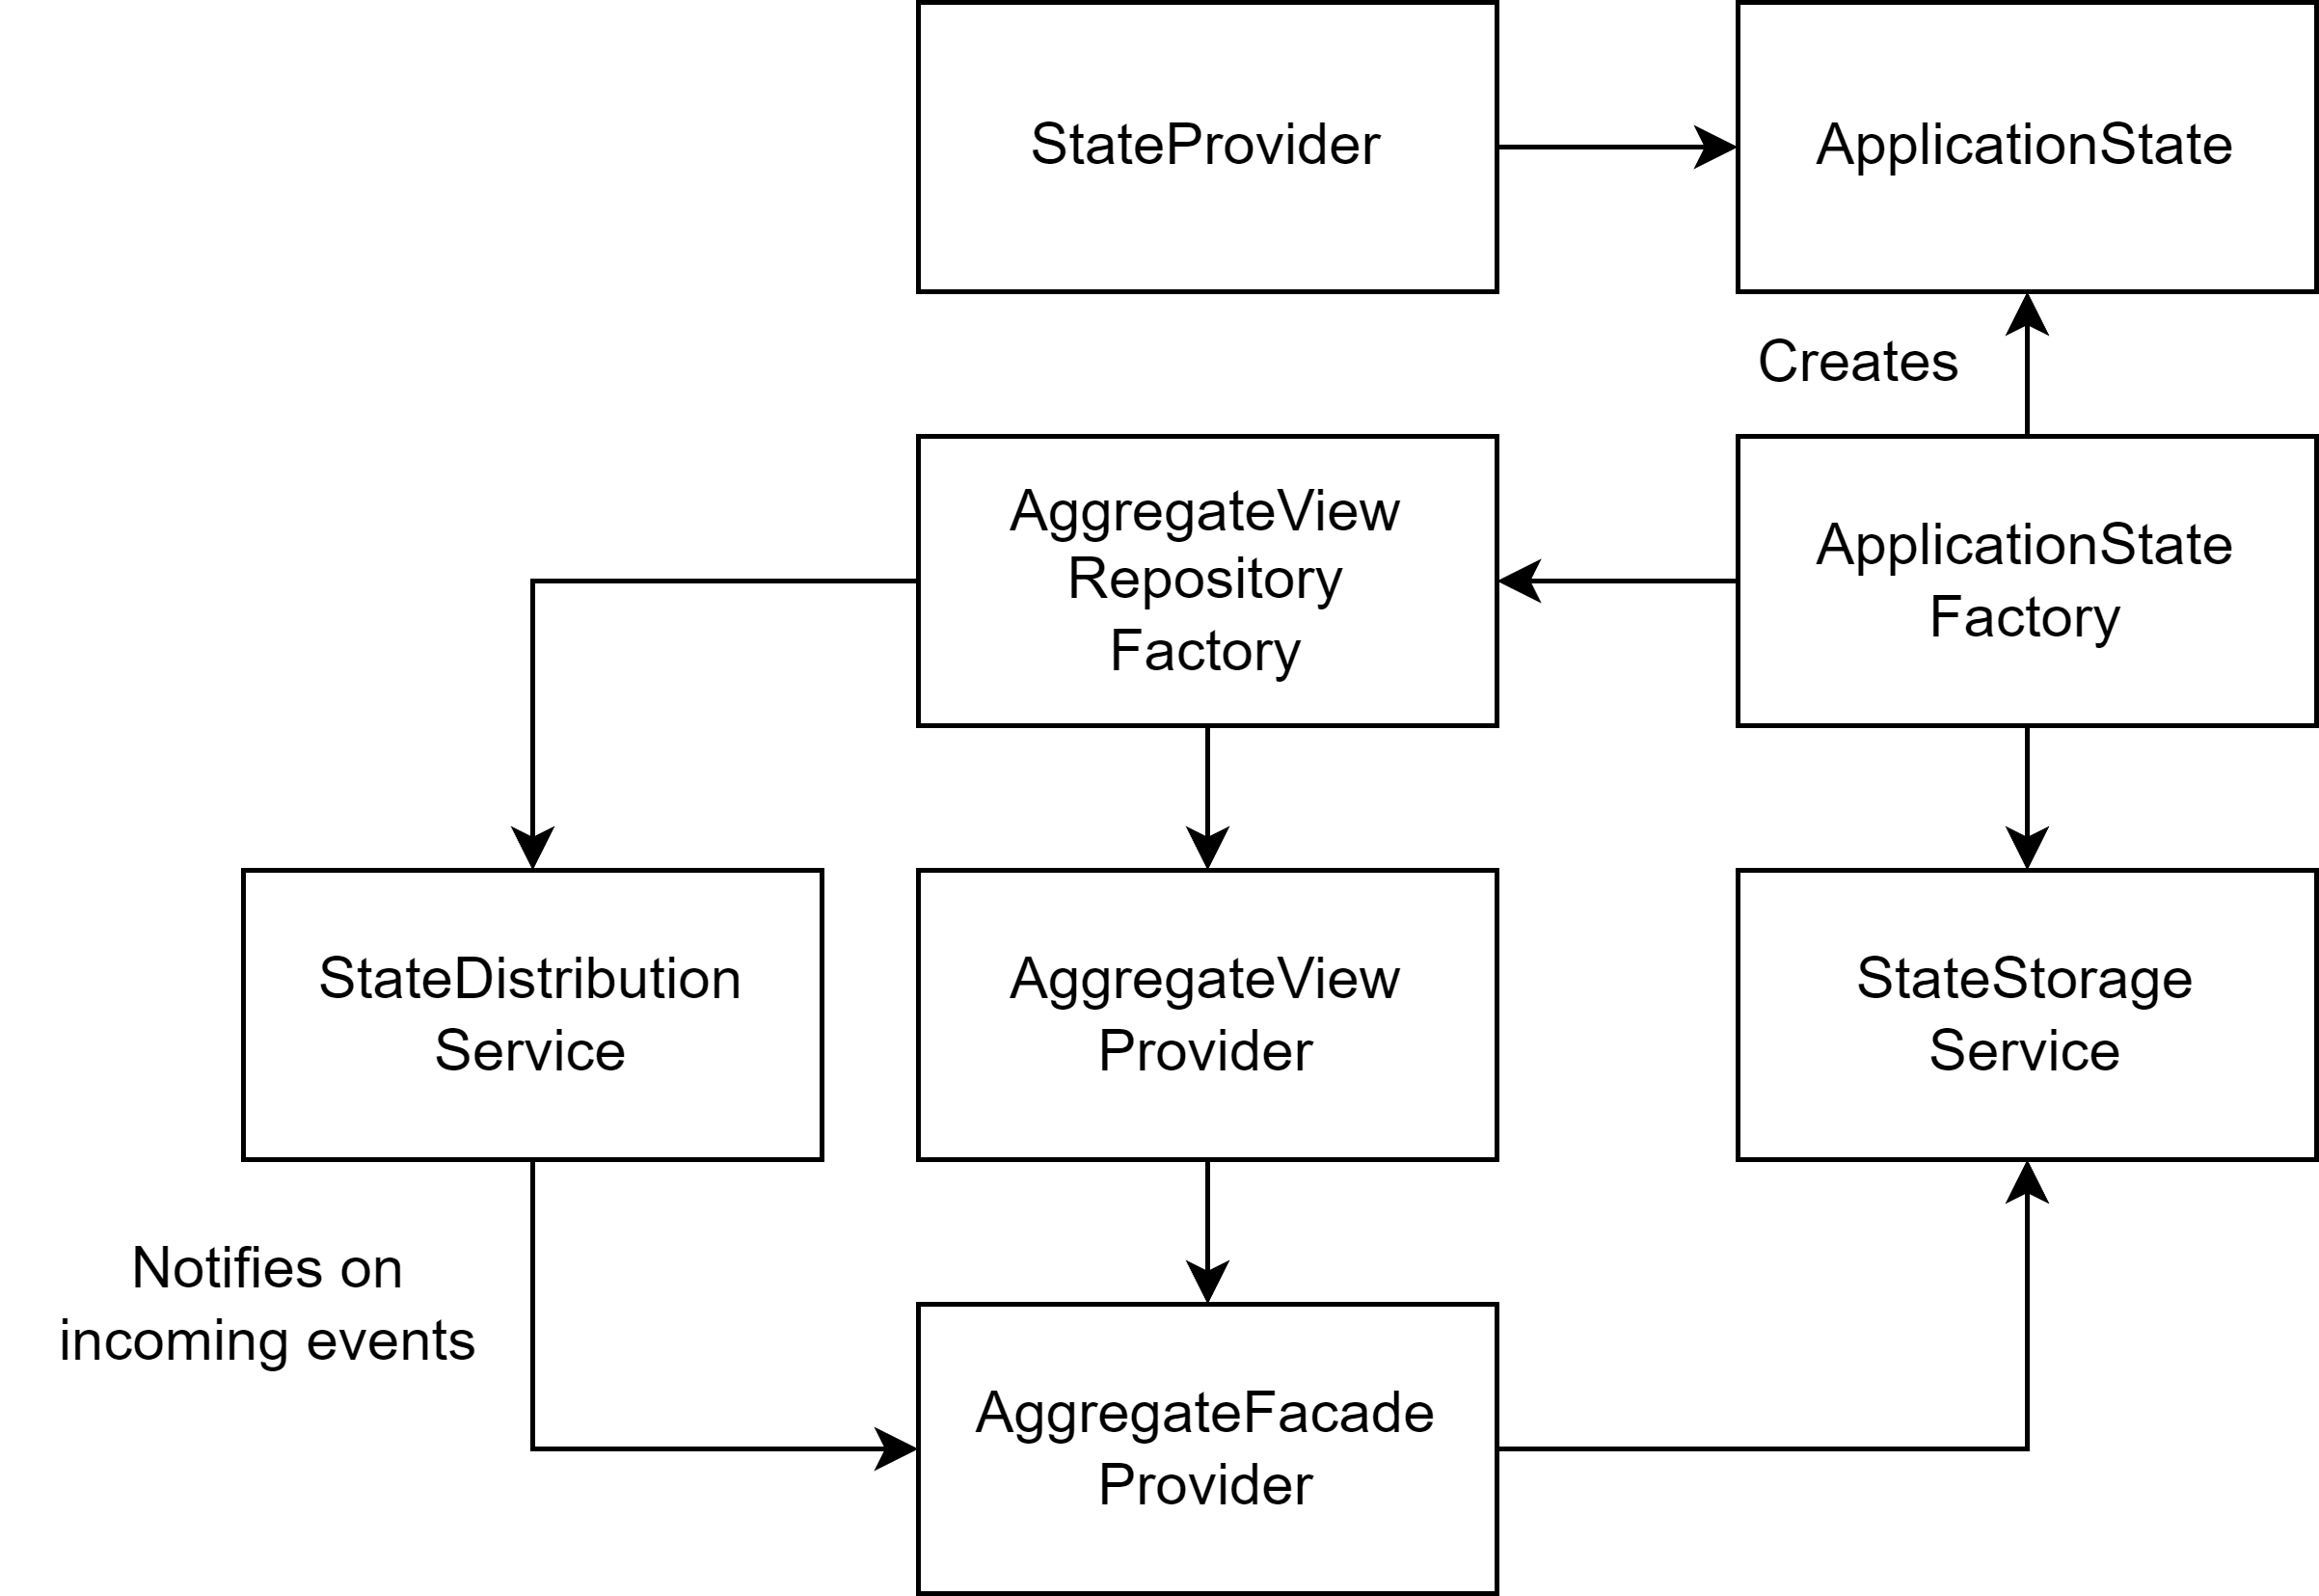
\includegraphics[width=0.7\textwidth]{state.png}
  \caption{Architecture overview}
\end{figure}

Access to the AggregateViewProvider is handled through AggregateViewRepositories which are created through the AggregateViewRepositoryFactory and then saved as ApplicationState. The separation between AggregationViewProvider and AggregateFacadeProvider is needed so that other state services can access the AggregateFacade instead of the AggregateView. The two services currently using this are the StateStorageService handling loading and saving aggregates on the user device and the StateDistributionService handling outgoing and incoming events. 

Using this abstraction we can now provide an ApplicationState like the following.

\begin{lstlisting}
case class ApplicationState(
  ratables: AggregateViewRepository[Ratable, RatableContext, RatableEvent],
  library: AggregateViewRepository[RatableLibrary, RatableLibraryContext, RatableLibraryEvent]
)
\end{lstlisting}

\chapter{Future}
Real peer to peer systems using ecmrdt's

Why do we have events and contexts. Couldnt we just say Event extends Context and explicitly associate them from the beginning?

Include event signing in general ECmRDT architecture.

- evaluation (ecmrdt als konzept messen -> speed, time)
- negative aspekte darstellen
- examples for ecmrdts
- Conclusion and future
- The ratable case study (title der case study)

\end{document}
